\documentclass[a4paper]{article}
\usepackage[spanish]{babel}
\usepackage{hyperref}
\usepackage{graphicx}
\usepackage{fancyhdr}
\usepackage[margin=3.5cm, top=2.5cm, bottom=3cm, includefoot]{geometry}
\usepackage{xcolor}


\graphicspath{ {imagenes3/} }

\setlength{\headsep}{2.5cm}
\pagestyle{fancy}
\fancyhf{}
\lhead{
\includegraphics[width=4cm]{Nuevo-Logo-1.jpg}}
\rfoot{{\textbf{Spark} \\ Master en Big Data y Data Science}}
\lfoot{ \break Página \thepage}
\renewcommand{\headrulewidth}{0pt}





\begin{document}
\begin{titlepage}
    \centering
    {\bfseries\LARGE Universidad Internacional de Valencia \par}
    \vspace{1cm}
    {\scshape\Large Master en Big Data y Data Science \par}
    \vspace{3cm}
    {\scshape\Huge Problema 3: Persona y método de pago. \par}
    \vspace{1cm}
    \begin{figure}[h]
        \centering
        
\includegraphics[width=8cm, keepaspectratio]{Nuevo-Logo-1.jpg}

    \end{figure}
    \vspace{1cm}
    {\itshape\Large Procesamiento de datos masivos: Spark \par}
    \vspace{3cm}
    {\Large Autor: \par}
    {\Large Adrián Hernández Padrón \par}
    {\Large Julio 2022 \par}


\end{titlepage}
\clearpage
\begin{section}{Código}
    Una vez se han leido los datos de entrada, vamos a mapearlos. Para ello creamos dos funciones, una que se encargue del saldo mayor de 1500 y otra que se encarge del saldo menor o igual a 1500. Como solo evaluamos el saldo en tarjetas de crédito tenemos que poner un condicional para que agregue 
    solamente las compras con tarjeta de crédito y también para cubrir el caso de cualquier persona que solo tenga compras sin tarjeta de crédito.

    El primer paso será dividir por línea la entrada y después, con un bucle, separar cada línea del fichero de entrada. Aplicamos el condicional y lo añadimos al array vacío en cada caso para tener la información correctamente mapeada con la clave-valor: nombre-1, de manera que podamos sumar luego los contadores.


    \begin{figure}[h]
        \centering
        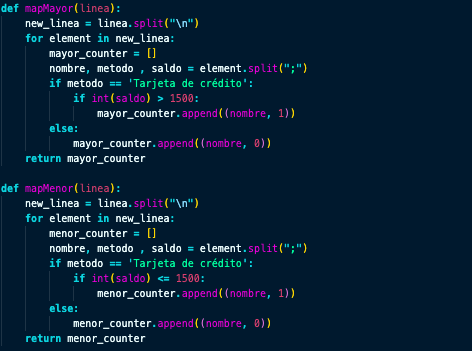
\includegraphics[width=\textwidth, keepaspectratio]{codigo1}
        \caption{El else se encarga de cubrir el caso de que una persona exista en el fichero pero no tenga compras con tarjeta de crédito.}

    \end{figure}
    
    Ahora usamos el flatmap y el reduceByKey para resolver el ejercicio, lanzando uno para las compras superiores a 1500 y otro para las inferiores.
    También nos ayudamos de un map para escribir los resultados con la estructura deseada.
\begin{figure}[h]
    \centering
    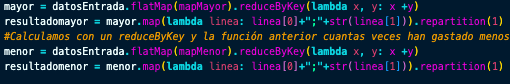
\includegraphics[width=\textwidth, keepaspectratio]{codigo2}

\end{figure}
\clearpage

    Y ya por último guardamos la salida en dos carpetas distintas.
    \begin{figure}[h]
        \centering
        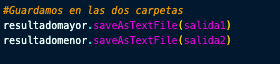
\includegraphics[width=\textwidth, keepaspectratio]{codigo3}
    \end{figure}
\end{section}

\begin{section}{Ejecución y resultados}
    Para lanzar el programa en este caso, escribimos lo siguiente por la linea de comandos: 
    $spark-submit personaYMetodosDePago.py file:/Users/adrihp/Master/MBID03/scriptsSpark/Problema3/entrada3.txt 
    file:/Users/adrihp/Master/MBID03/scriptsSpark/Problema3/comprasCreditoMayorDe1500 file:/Users/adrihp/Master/MBID03/scriptsSpark/Problema3/comprasCreditoMenorDe1500$

    en donde las últimas dos rutas hacen referencia a las dos carpetas en donde vamos a guardar la salida.

    La entrada y la salida del programa fueron las siguientes.
    \begin{figure}[h]
        \centering
        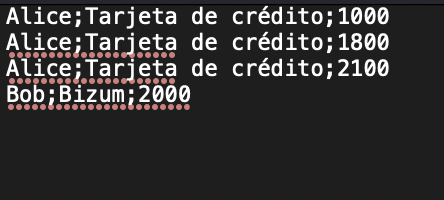
\includegraphics[width=\textwidth, keepaspectratio]{entrada3.png}
    \end{figure}
    \begin{figure}[h]
        \centering
        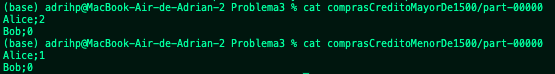
\includegraphics[width=\textwidth, keepaspectratio]{salida3.png}
    \end{figure}
    
\end{section}

\end{document}